
%(BEGIN_QUESTION)
% Copyright 2011, Tony R. Kuphaldt, released under the Creative Commons Attribution License (v 1.0)
% This means you may do almost anything with this work of mine, so long as you give me proper credit

One of the chemical processes used in some petroleum oil refineries to convert heavy oils into more marketable products such as jet fuel is called {\it hydrocracking}, where hydrogen gas is added to hot oil at very high pressure to ``crack'' the oil molecules into smaller (shorter-length) molecules that make lighter oils:

$$\includegraphics[width=15.5cm]{i00433x01.eps}$$

The hydrocracking reaction is exothermic, which means it produces (rather than absorbs) heat.  In order to control the reaction temperature and prevent it from ``running away,'' cool hydrogen gas is added to each catalyst bed inside the reactor to {\it quench} the reaction and regulate its temperature.

\vskip 10pt

Assuming all transmitters are direct-acting, determine the necessary actions of each controller in this system so that each control loop will be stable.  Note the valve actions for each loop:

\begin{itemize}
\item{} TV-5 = signal-to-open ; TIC-5 = {\it direct} or {\it reverse} action?
\item{} TV-6 = signal-to-open ; TIC-6 = {\it direct} or {\it reverse} action?
\item{} TV-7 = signal-to-open ; TIC-7 = {\it direct} or {\it reverse} action?
\item{} TV-9 = signal-to-open ; TIC-9 = {\it direct} or {\it reverse} action?
\item{} PV-13 = signal-to-close ; PIC-13 = {\it direct} or {\it reverse} action?
\end{itemize}

\vskip 20pt \vbox{\hrule \hbox{\strut \vrule{} {\bf Suggestions for Socratic discussion} \vrule} \hrule}

\begin{itemize}
\item{} For those who have studied chemistry, what property of hydrogen gas makes it such a good coolant?
\end{itemize}

\underbar{file i00433}
%(END_QUESTION)





%(BEGIN_ANSWER)

\begin{itemize}
\item{} TIC-5 = {\bf direct} action
\item{} TIC-6 = {\bf direct} action
\item{} TIC-7 = {\bf direct} action
\item{} TIC-9 = {\bf reverse} action
\item{} PIC-13 = {\bf reverse} action
\end{itemize}

%(END_ANSWER)





%(BEGIN_NOTES)


\filbreak \vskip 20pt \vbox{\hrule \hbox{\strut \vrule{} {\bf Virtual Troubleshooting} \vrule} \hrule}

\noindent
{\bf Predicting the effect of a given fault:} present each of the following faults to the students, one at a time, having them comment on all the effects each fault would produce.

\begin{itemize}
\item{} 
\item{} 
\item{} 
\end{itemize}


\vskip 10pt


\noindent
{\bf Identifying possible/impossible faults:} present symptoms to the students and then have them determine whether or not a series of suggested faults could account for all the symptoms, explaining {\it why} or {\it why not} for each proposed fault:

\begin{itemize}
\item{} Symptom: {\it }
\item{}  -- {\bf Yes/No}
\item{}  -- {\bf Yes/No}
\item{}  -- {\bf Yes/No}
\end{itemize}


\vskip 10pt


\noindent
{\bf Determining the utility of given diagnostic tests:} present symptoms to the students and then propose the following diagnostic tests one by one.  Students rate the value of each test, determining whether or not it would give useful information (i.e. tell us something we don't already know).  Students determine what different results for each test would indicate about the fault, if anything:

\begin{itemize}
\item{} Symptom: {\it }
\item{}  -- {\bf Yes/No}
\item{}  -- {\bf Yes/No}
\end{itemize}


\vskip 10pt


\noindent
{\bf Diagnosing a fault based on given symptoms:} imagine the hydrogen compressor fails to deliver an adequate flow of hydrogen gas to the reactor bed quench valves (don't reveal the fault to students!).  Present the operator's observation(s) to the students, have them consider possible faults and diagnostic strategies, and then tell them the results of tests they propose based on the following symptoms, until they have properly identified the nature and location of the fault:

\begin{itemize}
\item{} Operator observation: {\it TIC-5 below setpoint: SP = 625 $^{o}$F ; PV = 658 $^{o}$F and rising}
\item{} TIC-5 output = 100\%
\item{} TV-5 stem position = 100\% (wide open)
\item{} TIC-6 above setpoint: SP = 650 $^{o}$F ; PV = 689 $^{o}$F and rising ; Output = 100\%
\item{} TV-6 stem position = 100\% (wide open)
\item{} TIC-7 above setpoint: SP = 660 $^{o}$F ; PV = 705 $^{o}$F and rising ; Output = 100\%
\item{} TV-7 stem position = 100\% (wide open)
\item{} TIC-9 at setpoint: SP = 600 $^{o}$F ; PV = 599 $^{o}$F ; Output = 61\%
\item{} TI-10 = 605 $^{o}$F (this is normal)
\end{itemize}

%INDEX% Process: hydrocracker (oil refinery)

%(END_NOTES)


